\documentclass[11pt]{article}
% RFP specifically says to use 11 point type and 1 inch margins
\usepackage{graphicx}
\usepackage{epsf,color}
\textwidth=6.5in\oddsidemargin=0in \evensidemargin=0in \topmargin
0pt \advance \topmargin by -\headheight \advance \topmargin by
-\headsep \textheight 9.0in

%\textwidth=6.5in\oddsidemargin=0in \evensidemargin=0in \topmargin
%0pt \advance \topmargin by -\headheight \advance \topmargin by
%-\headsep \textheight 8.9in

\usepackage{amsmath}
\usepackage{graphicx}
\usepackage{dcolumn}
\usepackage{multirow}
\usepackage{wrapfig}
\usepackage[compact]{titlesec}

%\usepackage[plain]{fullpage}
\usepackage{amsfonts}
%\usepackage{lastpage}
%\usepackage{fancyhdr}

%\usepackage[version=3]{mhchem} 
% you can use this command to skip chunks of your document
% just put the command around the chunk like this
% \comment{ ...the chunk... }
\newcommand{\comment}[1]{}

%\newcommand{\MarginPar}[1]{\hspace{1sp}\marginpar{\tiny\sffamily\raggedright\hspace{1sp}#1}}
\setlength{\marginparwidth}{0.75in}
\newcommand{\MarginPar}[1]{\marginpar{%
\vskip-\baselineskip %raise the marginpar a bit
\raggedright\tiny\sffamily
\hrule\smallskip{\color{red}#1}\par\smallskip\hrule}}

%\renewcommand{\baselinestretch}{1.05} % = 1.0 Single space; = 2.0 Double
\renewcommand{\baselinestretch}{1.0} % = 1.0 Single space; = 2.0 Double

%\renewcommand{\refname}{Literature Cited}
%------------------------

%\pagestyle{empty}  % No page numbers
%\textfloatsep 0mm
%\abovecaptionskip 1mm

\begin{document}

%\pagestyle{plain}
%\pagenumbering{roman}
\begin{center}
{\large{\textbf{Combining Data and Simulation to Predict the Behavior of Complex Systems}}}

\vskip\baselineskip
%{\large{ Lead PI:  J. Bell \\
{{ Lead PI:  J. Bell \\
Senior Personnel: M. Day, J. Goodman, R. Grout, S. Habib, M. Kowalsky, M. Morzfeld, G. Pau}}
\end{center}

\subsection*{Background}

Predicting the behavior of complex physical systems is a key requirement for
many important DOE applications.
One approach to predicting the behavior of such systems is through high fidelity simulation. However,
for many systems uncertainties in the model used for computation limit its predictive capability.
Systems can also be probed experimentally; however, the 
relationship between the data and the system
can be complicated,
making it difficult to predict system behavior directly from data.
%
%Typically, these systems are investigated using a variety of different experiments, often
%aimed at probing a specific aspect of the physical system.
%However, the relationship between the data and the system
%can be complicated, requiring complex physics-based simulations to relate the data to underlying models.
%Futhermore, these simulations will depend on uncertain parameters describing
%the underlying physical system
%that must be simultaneously obtained from 
%the  experiments.
%
A third approach is to combine data with simulation. In particular, we want to use data from multiple experiments in conjunction with simulation to identify the range of model parameters that are consistent with the experimental data. This approach can reduce uncertainty in the model and therefore improve predictions of overall system behavior.
%Here, we propose to develop a methodology data and simulation to improve predictability,
%focusing on combustion modeling, cosmology and subsurface flow as motivating examples.
Here, we will
focus on combustion modeling, cosmology and subsurface flow as motivating examples.
However, the methodology will be broadly applicable to a
range of problems in chemical and materials science, systems biology, and climate to name a
few.

There are a number of common features shared by our target applications.
The systems are typically investigated using a variety of different experiments, often
aimed at probing different aspects of the behavior.
However, nonlinearity in the system dynamics makes it difficult to isolate the behavior of
a particular system component.
A second common feature is that there is a complex, often uncertain relationship between the state of the system and
what is being measured. For example, laser diagnostic measurements
of a chemical species in a reacting flow are modulated by quenching corrections that depend locally on the full
thermodynamic state of the system. Cosmological observations from telescopes provide a complex
space-time image  requiring corrections for
red shift and other effects. Data from tracer tests, resistivity measurements and pressure tests used to probe the subsurface
all provide complex nonlocal measurements of the system state. 
The third common characteristic of the systems we are considering is that the combination of the experiment not being sufficiently well defined 
and the dynamics being sufficiently complex means that we are often only trying to extract
statistical properties of the experiments, not a detailed trajectory.

The goal of this project is to develop a
mathematical framework for this class of problems that will allow us to use available data from a range
of experiments to restrict
uncertainty in the description of the system and estimate the impact of the improved characterization
on predictive capability.
We propose to address these issues using a combination of novel simulation and sampling methods that
intertwine parameter estimation and simulation into an integrated activity.

\subsection*{Approach}
We need an approach that allows us to pass
information through a range of experiments in a way that effectively uses all of the data
to improve overall predictive capabilities.
%Furthermore, as complexity increases,
%the combination of rich physics and relative data sparsity suggests that we will not be
%able to exactly match the experimental dynamics computationally.
We must develop estimation methods that are robust to model errors as well as partially unknown measurement processes.
The methodology needs to be able to use metrics based on identification of
characteristic features that are more general than
traditional quantities of interest.

To meet these requirements, we plan to use a Bayesian framework and assess via the posterior distribution how well system behavior
can be predicted based on all the data we have -- which aspects are tightly bounded and which are less precise. Our implementation will rely on Monte Carlo (MC) sampling to combine modeling and data in a way that provides full insight into the characterization of uncertainty of the complex system. Using MC sampling as the computational backbone leads to a numerically sound implementation that respects the strong nonlinearity in the target applications and is well suited to extreme-scale architectures, making this type of analysis possible for realistic applications.

%A core problem with current MC techniques is that they rely on prior sampling, which is problematic because,
%from a Bayesian perspective, high-probability events with respect to the prior are likely to have low
%probability with respect to the posterior. In short, the scaling of the number of prior samples with the number
%of dimensions of the problem is so poor that MC sampling is infeasible even for moderate scale problems;
%it is expected that large scale applications are still out of reach even when the number of samples can be
%increased dramatically by extreme-scale computing.
The key issue with a Bayesian approach is that current sampling techniques
are not robustly effective for complex, high-dimensional problems.
Standard particle filter methods break down in high dimensions because high-probability events 
with respect to the prior are likely to have low probability with respect to the posterior. 
Metropolis and heat bath algorithms suffer on problems that are poorly conditioned.
One of the central themes of this project will be to develop new smart sampling technologies 
to address these issues.
We will investigate the use of multigrid Markov chain Monte Carlo (MCMC) and parallel marginalization to reduce correlation
times and thus improve the effectiveness of sampling techniques.
We will also investigate the use of the implicit sampling methodology developed at LBNL.
Here, the central idea is to prevent the breakdown of particle filters by finding a probability distribution that approximates the
relationship between parameters and data. The search for a suitable approximate distribution is implemented
via solution of a minimization problem.
%When available we can use adjoint codes coupled to BFGS-type algorithms to solve the minimization problem
%using a parallel optimizer such as TAO from Argonne.
%\MarginPar{JG doubts this will work and notes a need to for derivative information to guide sampling. JBB
%doubts we can perform adjoint simulations for 3 turbulent simulations.  Only way out JB can think of
%is based on discussion with George about combining coarse simulation with a statistical surrogate to
%build an estimate of finer response . . . Unless someone has a brilliant idea here i suggest we leave this
%for the preproposal and thing of how to address it in real proposal}
%However, when adjoint codes are not available, derivative free optimization methods will be required.
%The most interesting and likely most successful type of approach here is a surrogate method,
%where a small number of forward simulations are utilized to generate a simplified model of the simulation.
This optimization can either be done using standard methods when a derivative (adjoint) is available
or with a derivative-free algorithm based on reduced order models (ROM).
Many research questions surround the interplay between optimization and
sampling, particularly with approximate surrogate models based on ROMs.

Effective sampling methodology must also deal with model degeneracy and inconsistency.
A model has an approximate degeneracy if many different parameter sets are nearly as good at explaining the data.
%For example, if there are multiple reaction pathways in a kinetic description,
%certain combinations of reaction rates may be much better
%estimated than the individual rates.
In such cases, isotropic sampling algorithms such as single variable heat bath (Gibbs sampler) or isotropic
Metropolis walk will be slow. We plan to use the affine sampling approaches developed at NYU to address issues of model degeneracy.
Methods must also be robust in the inevitable situation where the model is not consistent with the
data.
%For example, the power law/exponential formulas for reaction rates are only modeling approximations, though they can be
%very accurate.
In chaotic systems especially, even small modeling errors can make an accurate global fit impossible.
One approach is to include noise in the dynamics, so that the posterior distribution does not require the
dynamical equations to be satisfied exactly.
We will conduct computational experiments to study this problem, then use the results to 
choose appropriate noise levels for our physical models.
By combining what is known about the error levels in both model and data, we can estimate upper and lower bounds
of the predictive skills of the resulting stochastic models.

As noted above, ROMs can be used as
part of a derivative free optimization strategy
to guide a sampling procedure. We will also use ROMs to represent the mapping from the state of the system
to the data, especially when measurements are obtained from instruments with a complex and possibly uncertain response and for cases in which the data is statistical in nature. For these various purposes, different reduced order modeling techniques can be used, ranging from model reduction approaches for models with smooth solution manifolds, to response surface approaches or machine learning techniques for complex models.
%This analysis not only defines the predictive capability of the models, it also identifies
%the major factors that limit predictability and identify what additional data would most significantly
%impact the fidelity of predictions.

To evaluate the methodology we will examine test cases within each of our target application areas.
Specifically, we plan to consider how combustion experiments can be used to improve
the predictions of turbulent flames, how to use observations to improve our understanding of
cosmological parameters and how to use field scale measurements to improve prediction of subsurface
flows.
By adopting a Bayesian framework with MC sampling, the proposed methodology will provide an accurate representation of the posterior distribution that not only defines the limits of what can be predicted but also provides insight into how additional data could be used to improve fidelity. For the initial phases of the project, we plan to use synthetic data from high-fidelity simulations; however, for each target application we
plan to test the methodology with real data in the final year of the project.
\end{document}
%NEED SOMETHING ABOUT ROLE OF REDUCED ORDER MODELS.  I THINK ONE USE OF REDUCED ORDER
%MODELING IS TO GUIDE THE SMART SAMPLING APPROACHES IN MONTE CARLO.  ALSO SHOULD BE
%USEFUL IN SCALE BRIDGING BUT THAT IS MORE TENUOUS IN MY HEAD.

Examples:

\subsection*{Turbulence/Chemistry Interaction example:}

Inputs: Chemical kinetics and transport parameters with initial priors
 
Hierarchical data sources (experiments): 0d ignition, 1d laminar flames, shock-tube experiments
2D laminar flame DNS, 3D turbulent flames

Objectives:
\begin{itemize}
\item Use available data to reduce uncertainty in kinetics and transport
\item Estimate the impact of the improved characterization on predictive capability for turbulent flames
\item Identify which of the remaining uncertainties have the most impact on the uncertainty of the predictions
\end{itemize}
 
\subsection*{Point defect formation in thin-film photovoltaics:}
A key design need for high efficiency photovoltaic devices, e.g. those
based on CZTS absorbers, is the ability to control the carrier
concentration to achieve n+ and p+ doping resulting from point
defects. The creation of the various types of defects (intrinsic ionic
and electronic defects) can be described by a set of kinetic reaction
equations. For example, an abstract metal-sulfide system could be
described by simplistic system expressing an oxidation reaction, the
Schottky disorder and creation of anion vacancies:

\ce{ \tfrac{1}{2} S2 -> S_s^x + V_m^{''} + 2 h^+ }

\ce{ NULL -> V_m^{''}+ V_s^{$\cdot \cdot$} }

\ce{ NULL -> e^' + h^{$\cdot$} }

\ce{ S_s^x -> \tfrac{1}{2} S2 + V_s^{$\cdot \cdot$} + 2 e^- }

Near first-principles calculations such as electronic structure
calculations based on density functional theory can provide enthalpy
differences for the formation of these various point defects.
Neglecting the entropic contribution to the Gibbs energy, this
information is sufficient to determine equilibrium concentrations that
can be used to coarsely estimate the variation of the material
characteristics with the key parameters. For the system above, the
$S_2$ partial pressure is a key variable that when varied leads to a
Kroger-Vink diagram with the classic form shown in Figure~\ref{fig:kv}
where the crossover point between electron/hole concentrations is at
the stoichiometric pressure. \begin{figure}[h!]
  \centering
  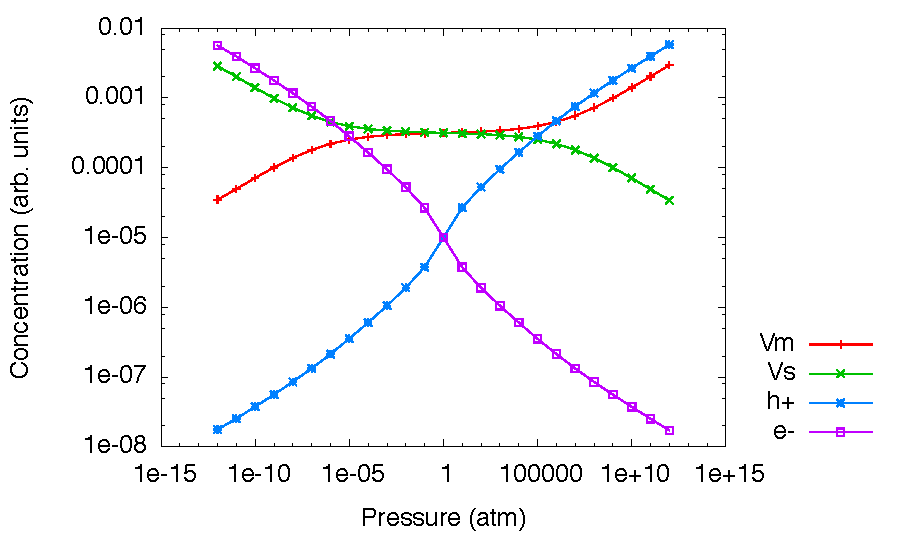
\includegraphics[width=0.8\textwidth]{KV.pdf}
  \caption{Kroger-Vink diagram for generic M-S system}
  \label{fig:kv}
\end{figure}
Even for this simplistic system, time-varying histories of the
non-metal pressure and temperature during crystal growth can be
expected to access quasi-equilibrium states. Additional parameters in
the Arrhenius forms for the kinetic rate expressions are required to
determine a time-dependent solution capable of predicting these states
with associated uncertainty. Complicating measurements that can be
used to estimate these parameters, diffusion of the non-metal species
($S_2$ above) into the film may be rate-limiting. Further, measurement
of the concentration of arbitrary point defects is difficult and must
be inferred from more easily observed characteristics. For realistic
systems, involving 10s to 100s of such kinetic expressions, many such
states with desirable properties may exist. Such states may be of
interest in two forms: firstly, they may useful for design of PV
systems, and secondly, they may have measurable characteristics that
allow us to reduce the uncertainty associated with one or more rates,
thereby allowing other states to be found that are useful for actual
devices.

In contrast to well-studied combustion chemical kinetics, where a
relatively (if still insufficient) quantity of experimental data points
have been acquired ti validate reaction mechanisms, point-defect systems are relatively poorly
understood. Many more experiments are necessary to converge on a
reasonable representation of the appropriate rates. 


FLESH OUT FROM RAY'S NOTES

\subsection*{Missing issues / concerns}

\begin{enumerate}
\item Need to flesh out more examples
\item How should we address the extreme-scale computing aspects of this
\item Fix general flakiness and flesh out places where help is needed
\end{enumerate}

\newpage

\section*{Matti's raw notes}


\begin{itemize}
\item Essentially all problems are non-linear and exhibit non-Gaussian statistics and, therefore, Monte Carlo sampling will be at the core of modern and next generation UQ techniques
\item Monte Carlo sampling is well suited for parallel computer architectures because the computationally expensive calculations (e.g. forward or adjoint/backward model runs) can be executed independently; the necessary communication happens only via scalar quantities, so that very little data must be moved across nodes
\item Due to a catastrophic scaling of the number of Monte Carlo simulations required with the number of dimensions of the underlying probability space, brute force Monte Carlo is not feasible for large-scale problems, even on exascale machines
\item New sampling techniques, developed at LBNL have shown promise in UQ in engineering problems (O(10) dimensions, e.g. in robotics, tracking of satellites) and in small scale geophysical inverse problems  (and their UQ, O(500) dimensions). The geophysical inverse problems are large enough such that traditional Monte Carlo is hopeless (on current and future machines).
\item We have experience with new sampling techniques for UQ, inverse problems and target tracking
\item The "technology" is ready for the next step: explore applicability to large/extreme scale problems, in particular (i) use of extreme scale minimization techniques (derivative free minimization, adjoint calculations, limited memory quasi-Newton methods); (ii) minimizing communication between cores/nodes and data movement/storage during sampling and updating; (iii) integration with large (extreme) scale simulation codes; (iv) a study of the scaling of the algorithm with the number of cores
\item Result: first large scale UQ system with smart Monte Carlo sampling and without Gaussianity or linearity assumptions
\item UQ  capabilities: UQ without Gaussianity or linearity assumptions; integration of experimental data and mathematical model/numerical codes; accurate tracking of uncertainty (e.g. covariances of errors); forecasting under uncertainty.

\end{itemize}


\section*{Ray's raw notes}

Thematic elements:

Manifold discovery / slow attractors

Link input parameters to changes in slow attractor

Identify observables based on characteristics of slow attractor that are related to changes in input parameters, specifically those we wish to investigate

Design framework so that each experiment conducted narrows the distribution of the priors to provide a strong probability of finding a change in attractors or measurable difference in output. 

Searching for transformation between distribution of inputs and distribution of outputs. 

Quantify the utility of an experiment by the degree of reduction in uncertainty

Use guided search based on priors to restrict the search space

Turbulence/Chemistry Interaction example:


Inputs: Chemical kinetics parameters, geometry, initial conditions

Traditional outputs: net overall burning rate in turbulent flame at device conditions

Candidates for optimal observable: reaction rate of each of n species, creation/destruction rates, vector indicating participation in each possible reaction pathway, vector indicating species participation.
(These are based on physical insight -- is it necessary to presuppose the candidates for observables?)
 
Data sources (experiments) hierarchy: 0d ignition simulation, 1d laminar flame simulation, library of 1d laminar flame experiments at conditions that perturb expected chemistry, ODT based laminar flame solution, 2D turbulent flame DNS, 3D turbulent flame DNS, shock tube ignition delay time parametric study.

Objective: Determine which chemical kinetics parameters to study further; design experiments with appropriate observables to objectively compare different kinetic mechanisms; design experiments to assess the impact of changing fuels (and hence mechanisms).

Point defect formation application:
Inputs: Potential kinetic mechanism; estimated activation energies based on DFT calculations; process conditions:

Observables: Quasi-equilibrium concentration of electrons in conduction band. 

Candidates for optimal observable: Individual point defect concentrations. 

Experimental hierarchy: Deterministic calculation of 0D equilibrium state, parametric in environmental conditions; experimental film growth with parametric variation of surface pressure, T (shifts relative rate of reactions); film growth in light/dark (may enable/disable defect formation mechanism); deterministic computation coupled to 1D transport; stochastic sampling of defect formation rates (using kinetic rates as transition probabilities).

Outcome: Determine process conditions that increase the probability of a favorable point defect configuration. Find the metastable states /attractors; assess these for favorable properties; engineer process likely to produce them. 

Other application areas:
\begin{itemize}
\item Anything with a reaction/kinetic network with uncertain parameters
\item Quantifying ``usefulness'' of expensive experiments
\item Kinetics of biological biomass deconstruction
\item Cosmology
\item OPV degradation rate modeling
\item Groundwater decontamination modelling 
\end{itemize}

Requisite features of application area:
\begin{itemize}
\item Model that can relate input parameters to observables with a hierarchy of fidelity
\item Targeted for kinetic reaction networks (conceivably this could be relaxed)
\item Dynamic / chaotic system with an underlying attractive manifold 
\item Finite number of attractors that can be described by continuous characteristics
\end{itemize}


%\newpage

\bibliographystyle{plain}

\bibliography{george_rom.bib} 



\end{document}
